\chapter{Results}\label{chapter:results}
Following the application of the event selection criteria, the training of the BDT and the evaluation of the BDT discriminant for the signal and background processes.


\section{Statistical Model}\label{sec:statisticalModel}
The calculation of 
Calculation of the observed signal strength, observed significance, and expected significance was performed  using the Higgs Analysis Combined Limit (\combine) tool~\cite{Combine}. 

The \combine tool is based on the RooStats package~\cite{Moneta:2010pm,Schott:2012zb} and determines the signal strength using a binned Maximum Likelihood Fit (MLF) and the significances using using an asymptotic approximation~\cite{AsymptoticFormulae}, using the Asimov dataset.



All systematic uncertainties were incorporated into the fit as nuisance parameters, with luminosity and fake rate taken as rate uncertainties and the remainder as shape uncertainties.
 
The fit was performed on the two channels simultaneously. 
Most systematics were assumed to be 100\% correlated between channels.

\subsection{Data-driven background normalisation}\label{subsec:combineNormalisation}

floating in the fit
\subsection{Treatment of Systematic Uncertainties}\label{subsec:combineNormalisation}


\section{Systematic Uncertainties}\label{chapter:systematics}
%%% Intro
For any meaningful and robust measurement to be made in any physics analysis, it is vital that the sources of systematic uncertainties associated with it are both understood and controlled.
This is particularly important when searching for tZq dilepton final state given that the high statistics of the background processes result in their systematic uncertainties being of a comparable order to the statistical uncertainties of the signal process.
Therefore without additional data to reduce the statistical uncertainty, the sensitivity of the search will be limited by the systematic uncertainties.

%%% Sources
These sources of uncertainty either originate from experimental or theoretical uncertainties and typically influence the result in one of two ways:
\begin{itemize}
\item \textbf{Rate or normalisation uncertainties} impact the number of events present and thus influence the  normalisation of the distributions considered.
\item \textbf{Shape or scale factor uncertainties} impact the shape of the distributions as they involve the scaling of individual events as a function of their kinematics in order to correct inconsistencies between simulation and data.
\end{itemize}

The statistical uncertainties arising from the size of the simulated samples available are also considered.

These uncertainties are treated as nuisance parameters in the statistical fit model which is described, along with the impact of the uncertainties on the result, in Chapter~\ref{sec:statisticalModel}.

\subsection{Experimental Uncertainties}
\subsubsection{Jet Energy Corrections}
The Jet Energy Corrections group also provides the uncertainties associated with the JES and JER they determine, discussed in Chapters~\ref{subsubsec:JECs} and~\ref{subsec:jesjer}, are determined by the Jet Energy Corrections group~\cite{Khachatryan:2016kdb}. 

The impact that the JES has on the jet kinematics is evaluated by varying the corrective JES up and down by a standard deviation.
The uncertainty associated with the JER smearing is accounted for by varying the smearing factor up and down by the associated statistical uncertainty.
Recently the uncertainties associated with the JER have been updated during the reprocessing of the 2016 dataset to include the systematic uncertainties in addition to the statistical uncertainties.
At the time of writing this thesis, these reprocessed samples and the impact of the revised total JER uncertainties has not been propagated through the analysis.

\subsubsection{\MET Uncertainties}
As \MET is calculated from the sum of the \pT of all the PF objects and the remaining unclustered energy deposits, the uncertainties associated from both have to be considered.

The impact of the uncertainties associated with both the JES and JER on the PF \MET are accounted for by propagating the JEC uncertainties through to the \MET and evaluating the impact they have.
As the unclustered energy remains uncorrected, the impact on the \MET uncertainty is evaluated by varying the difference between the \MET and total \pT of the PF objects up and down by 10\%, the default energy uncertainty.

During the time of writing this thesis, the method of determining the uncertainty associated with the unclustered energy was in the process of being replaced with a more precise method, where each particle is varied by its resolution.
Given the small impact of the \MET uncertainties, as discussed in Chapter~\ref{sec:uncertainitiesImpact}, it is anticipated that change will have a minimal impact on the final result.

\subsubsection{Pileup Reweighting}
The uncertainty associated with the primary vertex distributions used in the \PU reweighting is determined by varying the expected minimum bias cross section used in simulation $\pm X\%$ in order to ascertain the impact of greater or lesser amounts of \PU on the analysis.

\subsubsection{Parton Density Functions}\label{subsec:pdfSysts}
%%Discussion of what PDFs are, is given in an earlier chapter 
The impact of the PDF uncertainties are evaluated according to the PDF4LHC recommendations~\cite{Butterworth:2015oua}, where they are estimated as the standard deviation of the weights of the nominal and the variations of the PDF set.

For almost all of the MC samples considered, this is achieved by considering the nonimal event weight and one hundred alternative PDF weights which are stored as per-event weights in the LHE 
event header for almost all of the MC samples considered.

The single top tW-channel samples are the exception to this as at the time of their generation it was not possible to generate per-event weights to account for the PDF variations for this process.
Therefore, the LHAPDF (Les Houches Accord Parton Distribution Function) library is used to access both the nominal PDF weight and 50 eigenvalues from the NNPDF3.0 set to provide one hundred alternative event weights to be evaluated.

\subsubsection{b-tagging Uncertainties}
The uncertainties associated with the b-tagging scale factors described in Chapter~\ref{subsec:btagEff} are obtained by varying their value by $\pm 1\sigma$, as calculated by the BTV POG.

\subsubsection{Non-prompt Lepton Contributions}
The data-driven estimate of the instrumental backgrounds should have no dependence on either the lepton flavour or selection cuts.
Therefore the variation of the ratio of opposite-sign over same-sign events as a function of the lepton flavour and the cut level was considered to be well accounted for by a 30\% rate uncertainty.

\subsubsection{Z+jets Background}
As the aMC@NLO Z+jets sample is left to float in the fit, this accounts for the experimental normalisation systematic uncertainties.
The theoretical systematic uncertainties are accounted for as described in Chapter~\ref{sec:theorySysts}.

\subsubsection{Luminosity Uncertainties}
CMS uses the pixel detector, DTs, HF, the Fast Beam Conditions Monitor and Pixel Luminosity Telescope to monitor and measure the instantaneous and integrated luminosity.
During Run 2, the primary offline luminosity measurements made by the CMS Luminosity Group used the pixel detector using the Pixel Cluster Counting (PCC) method due its stability over time for up an average \PU of 150 and the high precision results obtained with it during Run I.
The PCC algorithm is able to achieve such a precision by measuring the instantaneous luminosity through the number of pixels present. 
This is possible as the probability of pixel hit belonging to multiple tracks is very small due to the very low occupancy of the detector, inferring that the number of pixel hits are linearly proportional to the number of interactions during a bunch crossing~\cite{CMS:2017_lumi}.

Using Van der Meer (VdM) scans during dedicated LHC runs to calibrate the absolute luminosity scale calibrations of the detectors~\cite{vanderMeer:1968zz}


The overall uncertainty in the integrated luminosity collected by CMS in 2016 was estimated to be 2.5\%~\cite{CMS:2017_lumi}.

%The MC events produced are weighted by a scale factor in order to correctly normalise them with respect to the data they are compared against.
%This normalisation scale factor is given by:
%\begin{equation}
%SF_{dataset} = \frac{\pazocal{L} \sigma}{N_{MC}^{Events}}
%\end{equation}
%where $\pazocal{L}$ is the amount of total integrated luminosity considered in the data used, $\sigma$ the cross section of the MC sample considered and $N_{MC}^{Events}$ is number of simulated events considered for the process.

\subsubsection{Lepton Efficiencies}
The uncertainties associated with the lepton identification, isolation and reconstruction efficiency scale factors discussed in Chapter~\ref{subsec:leptonRecoSFs} are varied +/- 1 sigma.

Several systematic studies were performed to estimate the systematic uncertainty for the trigger scale factors.
These studies included the comparison of the trigger efficiencies in simulation for \ttbar and Z+jets, the impacts of the \MET trigger selection and the further event selection in the analysis performed. 

\editComment{Elaborate once the impact of the potential changes to the trigger SFs are known}.


If both triggers are independent, then the efficiency of fulfilling both trigger selections can be expressed as:
\begin{equation}
\epsilon_{X + lepton triggers} = \epsilon_{X triggers} \times \epsilon_{lepton triggers}
\label{eq:triggerCorrelation}
\end{equation}

and if both trigger selections are uncorrelated, then the ratio of the left and right hand sides ($\alpha$) of Equation~\ref{eq:triggerCorrelation} would be 1.
Table~\ref{tab:triggerCorrelation} shows that the values of $\alpha$ determined for each channel only differ slightly from 1.


\begin{table}[htbp]
\topcaption {
The values of $\alpha$, expressing the strength of correlation between the lepton and cross triggers used to determine the trigger scale factors, for each channel.
}\label{tab:triggerCorrelation}
  \centering
  \resizebox{\textwidth}{!}{
% This right-aligns numbers in column, but centers them under column title.
 \begin{tabular}{cc}
   \hline
   \textbf{Channel} & \textbf{$\alpha$}   \\
   \hline   
   ee & 1.0 \\
   $\mu\mu$ & 1.0  \\
   e$\mu$ & 1.0  \\
   \hline
 \end{tabular}}
\end{table}

\subsection{Theoretical Uncertainties}\label{sec:theorySysts}

\subsubsection{Factorisation and renormalisation scales}
The factorisation and renormalisation scales ($\mu_{f}$,$\mu_{s}$) used at the Matrix Element and Parton Shower levels are parametrised as functions of $Q^{2}$.
In order to consider the impact of the uncertainty associated with the choice of scales used, $Q^{2}$ is varied up and down by factors of 2 and 0.5 respectively.

For the majority of the MC samples considered, the variations in $\mu_{f}$ and $\mu_{s}$ are stored in the LHE event header as per-event weights.
These weights are produced for where one scale is fixed as the other is varied or both are varied simultaneously.
The event weights for the simultaneously varied scales were used to reweighting each event in order to evaluate the impact of the $\mu_{f}$ and $\mu_{s}$ uncertainties.

In contrast to the ME level, the impact of the PS shower scale uncertainties was evaluated through the use of dedicated samples where the PS scale had been varied up and down.
These centrally produced samples are listed in Table~\ref{tab:theorySampleList} as the ``scale up'' and ``scale down'' samples.
In the case of \ttbar however, these samples are listed as ISR (initial-state radiation) and FSR (final-state radiation), as it includes the variations in the gluon emissions of the incoming and outgoing partons.

As mentioned above in Chapter~\ref{subsec:pdfSysts}, it was not possible for the single top tW-channel MC samples to be produced with per-event weights to account for the matrix element factorisation and renormalisation scales.
Dedicated samples for this process, listed in Table~\ref{tab:theorySampleList}, where the matrix element and parton shower scales are varied are used to evaluate these systematic uncertainties.

\subsubsection{Parton Shower Matching Thresholds}
As discussed in Chapter~\ref{subsec:eventGenerators}, all of the MC samples considered use model the hard scattering process through a dedicated Matrix Element generator, with PYTHIA 8 being used to perform the subsequent PS and hadronisation.

The uncertainty associated with the choice of the matching threshold used is evaluated by using the dedicated matching samples.
Such samples have been generated for the \ttbar and single top t-channel backgrounds, listed in Table~\ref{tab:theorySampleList}, where the model's matching threshold parameter \emph{hdamp} is varied up and down by one standard deviation~\cite{CMS:2016kle}.

\subsection{Impact of the Systematic Uncertainties}\label{sec:uncertainitiesImpact}
The effect of each of the sources of systematic uncertainty considered in terms of the pull ($\frac{ \hat{\theta} - \theta_{0} }{\Delta \theta}$) and the postfit impact of varying the sources of uncertainty by $\pm 1 \sigma$ are shown in figure~\ref{fig:systematicsPull}.

\editComment{Remark on the lumi, jer are the largest uncerts and how the rest of the experimental uncerts are considerably smaller}

\begin{figure}[htbp]
\begin{center}
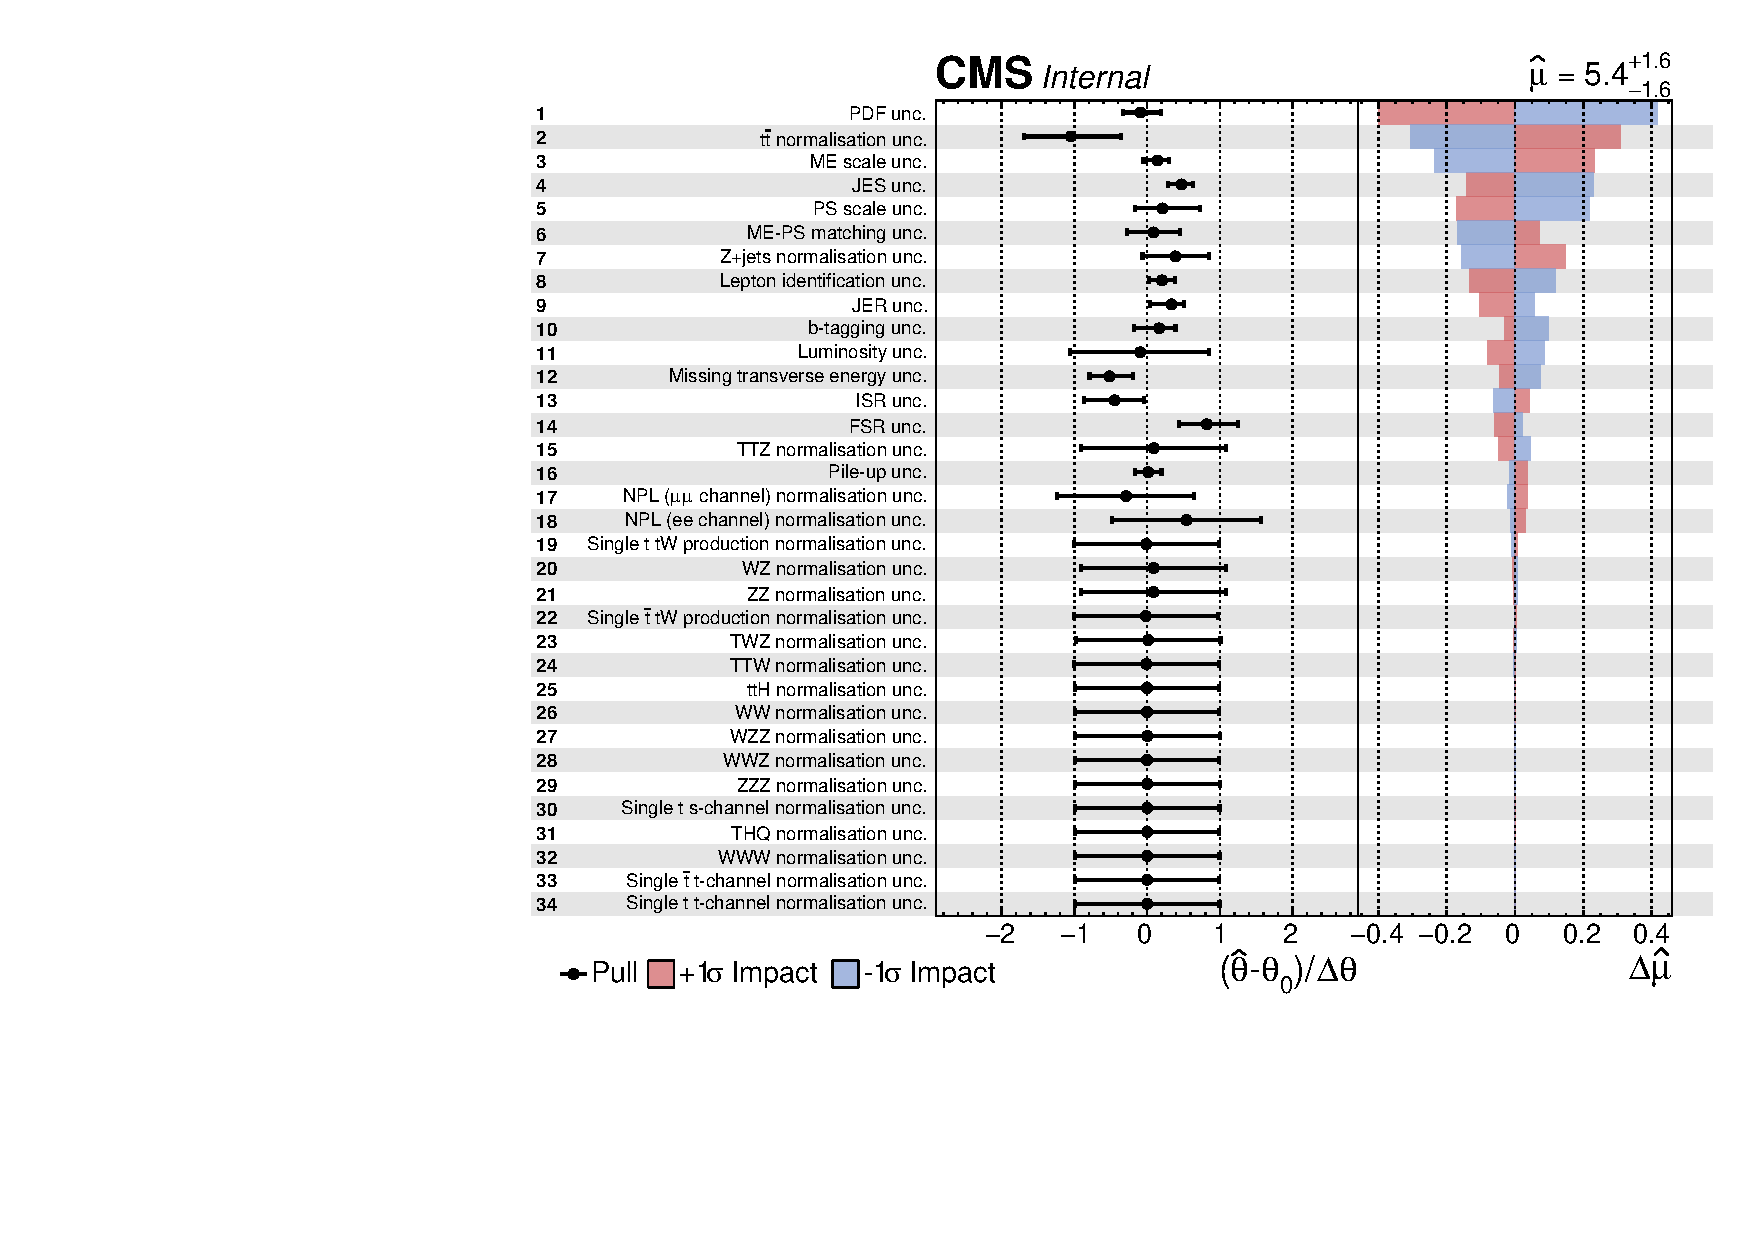
\includegraphics[width=0.97\textwidth]{figs/results/systematicsImpact.pdf}
\caption{The impact of each of the systematic uncertainties considered on the measurement made.}
\label{fig:systematicsPull}
\end{center}
\end{figure}

\section{Cross section extraction}
The cross section is 


By performing a simultaneous fit of the BDT discriminant distribution for the background-enriched sample and the BDT discriminant in the signal sample, any events in excess of the background-only hypothesis will be determined.

This excess can then be compared to the SM expectation for tZq production in order to calculate the observed signal strength and measure the cross section.

A measured signal strength of 0.0 would correspond to an observation of the background-only hypothesis alone, whilst 1.0 is the SM expectation for tZq sproduction.

\section{Signal strength significance}
The observed signal strengths, measured cross sections, and corresponding significances for the individual channels and the channels combined in the signal region using pseudo data, are shown in Table~\ref{tab:shapetxs}. 
These are [IN AGREEMENT / NOT IN AGREEMENT] with the SM cross section of  $X^{+Y}_{-Z}$.
 
\begin{table}[!h]
   \centering
   \caption{The observed signal strengths and corresponding cross sections for
   the individual channels and the channels combined at the 95\% CL.}
   \begin{tabular}{cccc}
       \hline
       Channel & $ee$ & $\mu\mu$ & \textbf{combination} \\
        \hline
        % \multicolumn{4}{c}{\combine{}} \\
        % \hline
        Signal strength & $X_{-Z}^{+Y}$ & $X_{-Z}^{+Y}$ & $X_{-Z}^{+Y}$ \\
       Cross section (fb) & $X_{-Z}^{+Y}$ & $X_{-Z}^{+Y}$ & $X_{-Z}^{+Y}$ \\
       Significance (expected) & $X_{-Z}^{+Y}$ & $X_{-Z}^{+Y}$ & $X_{-Z}^{+Y}$ \\
       Significance (observed) & $X_{-Z}^{+Y}$ & $X_{-Z}^{+Y}$ & $X_{-Z}^{+Y}$ \\
        \hline
        % \multicolumn{4}{c}{\textsc{Theta}} \\
        % \hline
        % Signal strength & $X_{-Z}^{+Y}$ & $X_{-Z}^{+Y}$ & $X_{-Z}^{+Y}$ \\
        % Cross section (fb) & $X_{-Z}^{+Y}$ & $X_{-Z}^{+Y}$ & $X_{-Z}^{+Y}$ \\
        % Significance (expected) & $X_{-Z}^{+Y}$ & $X_{-Z}^{+Y}$ & $X_{-Z}^{+Y}$ \\
        % Significance (observed) & $X_{-Z}^{+Y}$ & $X_{-Z}^{+Y}$ & $X_{-Z}^{+Y}$ \\
        % \hline
    \end{tabular}
   \label{tab:shapetxs}
\end{table}


\section{Interpretation of the results}

\section{Other results from the Large Hadron Collider}
The search for a singly produced top in association with a Z boson in the dilepton final state presented is the first one made at the LHC and follows in the footsteps of the searches for the trilepton final state at $\sqrt{8}$ and $\sqrt{13}$ using data collected by the CMS experiment in 2012 and 2016 respectively.

Despite the dilepton final state having a larger cross section than the trilepton final state, the different final state topology makes it much more difficult to isolate the signal process.
Consequently, the \editComment{expected/observed} significance of $A$ is smaller than the significances observed for the trilepton final state by CMS~\cite{Sirunyan:2017nbr} and ATLAS~\cite{Aaboud:2017ylb} at $\sqrt{13}$.
